\documentclass[11pt]{article}
\usepackage{fontspec}
\setmainfont{DejaVu Serif}
\usepackage{amsmath,amssymb}
\usepackage{geometry}\geometry{margin=2.3cm}
\usepackage{xcolor}\usepackage{graphicx}\usepackage{enumitem}\usepackage{booktabs}
\usepackage[hidelinks]{hyperref}
\definecolor{ink}{HTML}{16212e}\definecolor{accent}{HTML}{1f5fa8}\definecolor{soft}{HTML}{eef3fb}
\definecolor{warn}{HTML}{a8341f}\definecolor{good}{HTML}{16a34a}
\color{ink}
\newcommand{\key}[1]{\par\medskip\noindent\colorbox{soft}{\parbox{\dimexpr\linewidth-2\fboxsep}{\textcolor{accent}{\textbf{Κλειδί:}}\ #1}}\par\medskip}
\newcommand{\ex}[1]{\par\smallskip\noindent\textbf{\textcolor{accent}{Παράδειγμα.}}\ #1\par\smallskip}
\newcommand{\analogy}[1]{\par\smallskip\noindent\textit{\textbf{Αναλογία:}\ #1}\par\smallskip}
\newcommand{\warnb}[1]{\par\medskip\noindent\colorbox{soft}{\parbox{\dimexpr\linewidth-2\fboxsep}{\textcolor{warn}{\textbf{Προσοχή:}}\ #1}}\par\medskip}
\setlength{\parskip}{0.5em}\setlength{\parindent}{0pt}

\title{\textbf{Φροντιστήριο: Πώς δουλεύει το Deep Momentum δίκτυό μας}\\[3pt]
\large Από τον απλό κανόνα στο νευρωνικό δίκτυο --- και γιατί η διασπορά αποφασίζει\\[-1pt]
\normalsize\textcolor{accent}{DMN/LSTM $\cdot$ attention $\cdot$ Sharpe-loss $\cdot$ leak-free walk-forward $\cdot$ ENB $\cdot$ Deflated Sharpe}}
\author{QUANTIQ / AGEL AI --- Stefanos Drakos}\date{\today}

\begin{document}
\maketitle\thispagestyle{empty}

\noindent Φτιάξαμε ένα \textbf{νευρωνικό δίκτυο} που μαθαίνει μόνο του πότε και πόσο να αγοράζει/πουλά,
και το συγκρίναμε με έναν \textbf{απλό κανόνα}. Αυτό το κείμενο εξηγεί από την αρχή, για αρχάριο, τι
κάνει το καθένα, πώς το ελέγξαμε \emph{τίμια}, και το πιο σημαντικό μάθημα: \textbf{ένα πιο εξελιγμένο
μοντέλο δεν είναι αυτόματα καλύτερο}. Όλα τα νούμερα είναι από τα δικά μας πραγματικά πειράματα
(paper5, δωρεάν Yahoo δεδομένα, daily, net των πραγματικών eToro κοστών).

\tableofcontents
\bigskip

\section{Τι θέλουμε να πετύχουμε}
\textbf{Momentum} = «ό,τι ανεβαίνει σταθερά, τείνει να συνεχίσει· ό,τι πέφτει, να συνεχίσει να πέφτει».
Άρα: αγόρασε ό,τι έχει ανοδική τάση, πούλα (short) ό,τι έχει καθοδική. Για να το παίξεις χρειάζεσαι
\textbf{δύο} αποφάσεις: (α) \emph{πώς} μετράς την τάση, (β) \emph{πόσα} βάζεις. Ο απλός κανόνας τις
ορίζει με το χέρι. Το δίκτυο προσπαθεί να τις \textbf{μάθει} από τα δεδομένα.

\section{Ο απλός κανόνας (το «baseline»)}
Ο κανόνας μας: κοίτα την τάση 120 ημερών (\texttt{sign} της απόδοσης), βάλε θέση \textbf{αντιστρόφως
ανάλογη της μεταβλητότητας} (μικρή θέση σε ταραγμένη αγορά), και \textbf{μην αλλάζεις θέση για μικρές
κινήσεις} (no-trade band). Είναι λίγες γραμμές, χωρίς «μάθηση».
\key{Αυτός ο απλός κανόνας είναι ο αντίπαλος που πρέπει να νικήσει το ML. Στα crypto daily δίνει net
IR \textbf{1.24} --- πολύ δυνατός.}

\section{Το Deep Momentum Network (DMN) --- το LSTM}
Αντί να ορίζουμε εμείς τάση+μέγεθος, αφήνουμε ένα \textbf{LSTM} (νευρωνικό δίκτυο με «μνήμη») να τα
μάθει μαζί και να βγάζει κατευθείαν μια \textbf{θέση} από $-1$ (πλήρως short) έως $+1$ (πλήρως long).
\analogy{Το LSTM διαβάζει τις τιμές των τελευταίων μηνών σαν αναγνώστης που θυμάται τα προηγούμενα
κεφάλαια για να καταλάβει το τωρινό.}

\subsection{Το έξυπνο κόλπο: εκπαιδεύεται στο \emph{κέρδος}, όχι στην \emph{πρόβλεψη}}
Τα συνηθισμένα μοντέλα μαθαίνουν να «προβλέπουν την τιμή». Το DMN \textbf{όχι}: εκπαιδεύεται να
μεγιστοποιεί απευθείας το \textbf{Sharpe} (κέρδος ανά ρίσκο) της στρατηγικής.
\analogy{Δεν μαθαίνεις τον ποδοσφαιριστή «να προβλέπει πού θα πάει η μπάλα», αλλά «\textbf{να σκοράρει
γκολ}». Μπορείς να έχεις 90\% σωστές προβλέψεις και να χάνεις λεφτά. Μόνο το κέρδος-ανά-ρίσκο μετράει.}
\key{Στο momentum χάνεις πιο \emph{συχνά} απ' ό,τι κερδίζεις, αλλά πιάνεις τα λίγα μεγάλα trends. Άρα
το «ποσοστό επιτυχίας» είναι άχρηστος στόχος --- μόνο το Sharpe.} Κρατάμε και το \textbf{vol-scaling}
(μικρή θέση σε ταραγμένη αγορά) και έναν όρο που \textbf{τιμωρεί το υπερβολικό trading} (κόστη).

\section{Τα 10 «μάτια» του δικτύου (features)}
Το δίκτυο δεν βλέπει την ωμή τιμή· βλέπει 10 κανονικοποιημένα σήματα ανά asset/μέρα:
\begin{center}\small
\begin{tabular}{cl}
\toprule
\# & Τι λέει (απλά) \\
\midrule
1--5 & Τάση σε 5 ορίζοντες (1/21/63/126/252 μέρες), διά τη μεταβλητότητα \\
6 & Πόσο ταραγμένη είναι η αγορά (log μεταβλητότητα) \\
7--9 & Κρυφή τάση (Kalman): ταχύτητα, σιγουριά, «έκπληξη» \\
10 & Πιθανότητα να \emph{άλλαξε το καθεστώς} της αγοράς (BOCPD, «έξυπνο φρένο») \\
\bottomrule
\end{tabular}
\end{center}

\section{Το attention (Momentum Transformer)}
Πιο εξελιγμένη αρχιτεκτονική: αντί να διαβάζει σειριακά, το attention κοιτάζει \textbf{όλο} το παρελθόν
και \emph{διαλέγει πού να εστιάσει}.
\analogy{Οδηγός σε ομίχλη: αντί να θυμάται μόνο τα τελευταία ήρεμα χιλιόμετρα, λέει «αυτό μοιάζει με την
ομίχλη του περασμένου χειμώνα» --- βρίσκει το \emph{σχετικό} παρελθόν, όχι απλώς το πρόσφατο.}
\warnb{Το attention είναι \textbf{πεινασμένο για δεδομένα}. Με λίγες μπάρες δεν προλαβαίνει να μάθει
καλά --- το θυμόμαστε γιατί παίζει ρόλο στα αποτελέσματα.}

\section{Leak-free nested walk-forward --- ο τίμιος έλεγχος}
Δεν εκπαιδεύουμε σε όλα τα δεδομένα και μετά «ελέγχουμε» στα ίδια (αυτό είναι ζαβολιά). Χωρίζουμε τον
χρόνο σε κομμάτια: σε κάθε βήμα εκπαιδεύουμε \textbf{μόνο στο παρελθόν} και ελέγχουμε στο επόμενο,
\emph{αδίδακτο} κομμάτι.
\analogy{Εξετάσεις κάθε χρόνο, όπου ο μαθητής έχει διαβάσει μόνο τις προηγούμενες χρονιές. Ποτέ δεν
βλέπει τις απαντήσεις πριν γράψει.}

\subsection{Γιατί ΔΕΝ αποθηκεύουμε τα βάρη του μοντέλου}
Σε ένα τίμιο walk-forward δεν υπάρχει «ένα» μοντέλο --- υπάρχουν πολλά, ένα ανά κομμάτι, και το καθένα
ισχύει μόνο για το δικό του παράθυρο. Για τον \textbf{έλεγχο} κρατάμε μόνο τις \textbf{θέσεις} (τι αγόρασε
κάθε μέρα) και τις πραγματικές αποδόσεις· από αυτά βγαίνουν όλα τα νούμερα.
\analogy{Για να βαθμολογήσεις ένα γραπτό χρειάζεσαι τις \textbf{απαντήσεις} του μαθητή και τις
\textbf{σωστές} απαντήσεις --- όχι το μυαλό του. Οι απαντήσεις είναι ήδη γραμμένες στο χαρτί.}
\key{Τα βάρη χρειάζονται μόνο για \emph{live trading} (να βγάλεις θέση για το αύριο, που δεν υπάρχει
ακόμα). Για backtest αρκούν οι παγωμένες θέσεις. Αναπαραγωγιμότητα: ίδιος κώδικας + ίδιο seed
$\Rightarrow$ ίδια νούμερα.}

\section{Deflated Sharpe (DSR) --- τιμωρία για τις πολλές δοκιμές}
Αν δοκιμάσεις 100 παραλλαγές, κάποια θα φανεί καλή \emph{από τύχη}. Το DSR «ξεφουσκώνει» το Sharpe
ανάλογα με το \textbf{πόσες} ρυθμίσεις δοκίμασες.
\analogy{Αν ρίξεις 100 κέρματα, κάποιο θα φέρει 8 συνεχόμενες κορώνες. Δεν είναι «τυχερό κέρμα» ---
απλώς έριξες πολλά. Το DSR το λαμβάνει υπόψη.} DSR κοντά στο 1 = δύσκολα τύχη· κοντά στο 0 = ύποπτο.

\section{Διασπορά $>$ πλήθος --- το τεστ ENB (το κλειδί όλης της ιστορίας)}
Δύο assets που κινούνται μαζί (συσχέτιση $\approx 0.9$) είναι \textbf{ένα} στοίχημα, όχι δύο. Μετράμε
τον \textbf{πραγματικό αριθμό ανεξάρτητων στοιχημάτων} (ENB) από τον πίνακα συσχέτισης:
\[ \mathrm{ENB}=\frac{(\sum\lambda)^2}{\sum\lambda^2}\quad(=N\ \text{αν όλα ασυσχέτιστα},\ \to 1\ \text{αν όλα ίδια}). \]
\begin{center}\small
\begin{tabular}{lrr}
\toprule
Basket & μέση \textbar συσχέτιση\textbar & \textbf{ENB (πραγματικά bets)} \\
\midrule
8 crypto & 0.52 & \textcolor{warn}{2.6 / 8} (33\%) \\
18 crypto+ETF & 0.26 & \textcolor{good}{6.1 / 18} (34\%) \\
\bottomrule
\end{tabular}
\end{center}
\begin{center}
\includegraphics[width=\linewidth]{figures/fig_diversification.png}\end{center}
\key{Τα 8 crypto καταρρέουν σε μόλις \textbf{2.6} πραγματικά στοιχήματα (όλα ακολουθούν το BTC). Το
Sharpe-loss του δικτύου, που \emph{ζει από τη διασπορά}, μένει χωρίς σήμα --- γι' αυτό το δίκτυο
καταρρέει. Με 18 assets τα bets υπερδιπλασιάζονται σε \textbf{6.1}.}

\section{Τα αποτελέσματα}
\textbf{(α) Μόνο crypto (8 assets, ENB 2.6) --- τίμιος null:}
\begin{center}\small
\begin{tabular}{llrrrl}
\toprule
μοντέλο & band & net IR & NW-t & DSR & +2022 \\
\midrule
απλός κανόνας & hard & \textbf{1.24} & 2.73 & 1.00 & ναι \\
LSTM-DMN & none & 0.07 & 0.16 & 0.16 & όχι \\
LSTM-DMN & hard & 0.37 & 0.82 & 0.43 & όχι \\
Transformer & none & 0.07 & 0.20 & 0.26 & όχι \\
Transformer & hard & 0.04 & 0.11 & 0.23 & ναι \\
\bottomrule
\end{tabular}
\end{center}
Το ML \textbf{κατέρρευσε} (net IR $\approx 0$, στατιστικά ασήμαντο). Ο απλός κανόνας κερδίζει συντριπτικά.

\textbf{(β) Crypto + ETF (18 assets, ENB 6.1) --- η διάγνωση επιβεβαιώνεται:}
\begin{center}\small
\begin{tabular}{llrrrl}
\toprule
μοντέλο & band & net IR & NW-t & DSR & +2022 \\
\midrule
απλός κανόνας & hard & \textbf{1.11} & 2.32 & 1.00 & ναι \\
LSTM-DMN & none & \textcolor{good}{0.92} & 1.59 & 0.86 & όχι \\
LSTM-DMN & hard & 0.88 & 1.55 & 0.84 & όχι \\
Transformer & none & 0.07 & 0.14 & 0.24 & όχι \\
Transformer & hard & 0.05 & 0.12 & 0.23 & όχι \\
\bottomrule
\end{tabular}
\end{center}
\begin{center}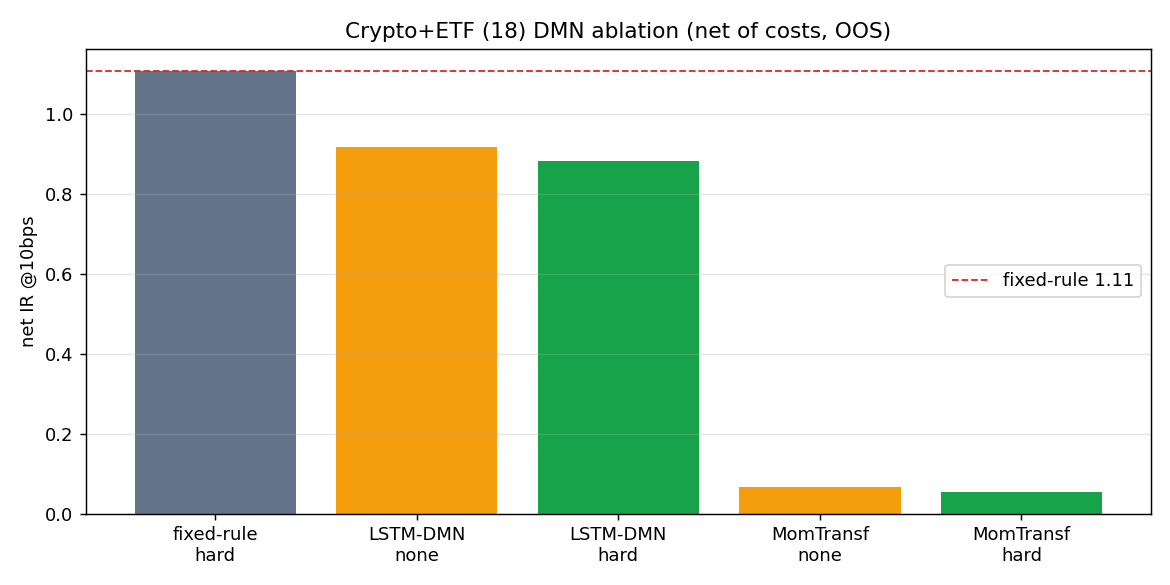
\includegraphics[width=0.92\linewidth]{figures/fig_dmn_combined.png}\end{center}
\key{Το LSTM-DMN \textbf{εκτοξεύτηκε 0.07 $\to$ 0.92} μόνο με διασπορά (ENB 2.6 $\to$ 6.1) --- από
«νεκρό» έγινε ανταγωνιστικό. Επιβεβαιώνεται ότι ο crypto-only null ήταν artifact λεπτού universe.}

\section{Πώς διαβάζεται ο πίνακας}
\textbf{net IR}: κέρδος-ανά-ρίσκο (πάνω από $\sim$0.8 αξιοπρεπές, $>$1 πολύ καλό). \textbf{NW-t}: σιγουριά
ότι δεν είναι τύχη ($>$2 σημαντικό). \textbf{DSR}: όπως το t αλλά τιμωρεί τις πολλές δοκιμές.
\textbf{+2022}: κέρδισε μέσα στο crash; (αντοχή σε bear).

\section{Τα τρία μαθήματα}
\textbf{1. Διασπορά $>$ πλήθος.} Ο μοχλός για το ML δεν είναι ο αριθμός των assets αλλά τα \emph{ανεξάρτητα}
στοιχήματα (ENB). 6.1 ξύπνησαν το δίκτυο, 2.6 το σκότωσαν.

\textbf{2. Το attention θέλει πολλά δεδομένα.} Ο Transformer έμεινε νεκρός (0.05--0.07) ακόμα και
διαφοροποιημένος: $\sim$3000 μπάρες δεν φτάνουν. Το \textbf{χαμηλότερης χωρητικότητας LSTM} είναι πιο
αποδοτικό σε λίγα δεδομένα.

\textbf{3. Πιο εξελιγμένο $\ne$ καλύτερο.} Παραπάνω «δύναμη» χωρίς αντίστοιχη πολυπλοκότητα στο πρόβλημα
απλώς προσαρμόζεται στον θόρυβο.
\analogy{Στο «2+2» ένας καθηγητής με διδακτορικό δεν τα πάει καλύτερα από μαθητή δημοτικού --- ίσως
χειρότερα, αν ψάχνει παγίδες που δεν υπάρχουν.}
\key{Τελική τίμια ετυμηγορία: σε δωρεάν δεδομένα το ML \textbf{αναβιώνει με διασπορά} αλλά \textbf{δεν
νικά} τον καλο-φτιαγμένο απλό κανόνα (0.92 vs 1.11). Ο τίμιος null/near-miss \emph{είναι} το αποτέλεσμα
--- δεν το μακιγιάρουμε.}

\end{document}
